\documentclass[prodmode,acmtecs]{acmsmall}
\usepackage[ruled]{algorithm2e}
\renewcommand{\algorithmcfname}{ALGORITHM}
\SetAlFnt{\small}
\SetAlCapFnt{\small}
\SetAlCapNameFnt{\small}
\SetAlCapHSkip{0pt}
\IncMargin{-\parindent}

\usepackage{makeidx}
\usepackage{tabularx}
\usepackage{graphicx}
\usepackage{color}
\usepackage{pdfpages}
\usepackage{listings}    
\usepackage{float}
 \usepackage{url}
% Metadata Information
\acmVolume{9}
\acmNumber{4}
\acmArticle{1}
\acmYear{2010}
\acmMonth{3}

\begin{document}
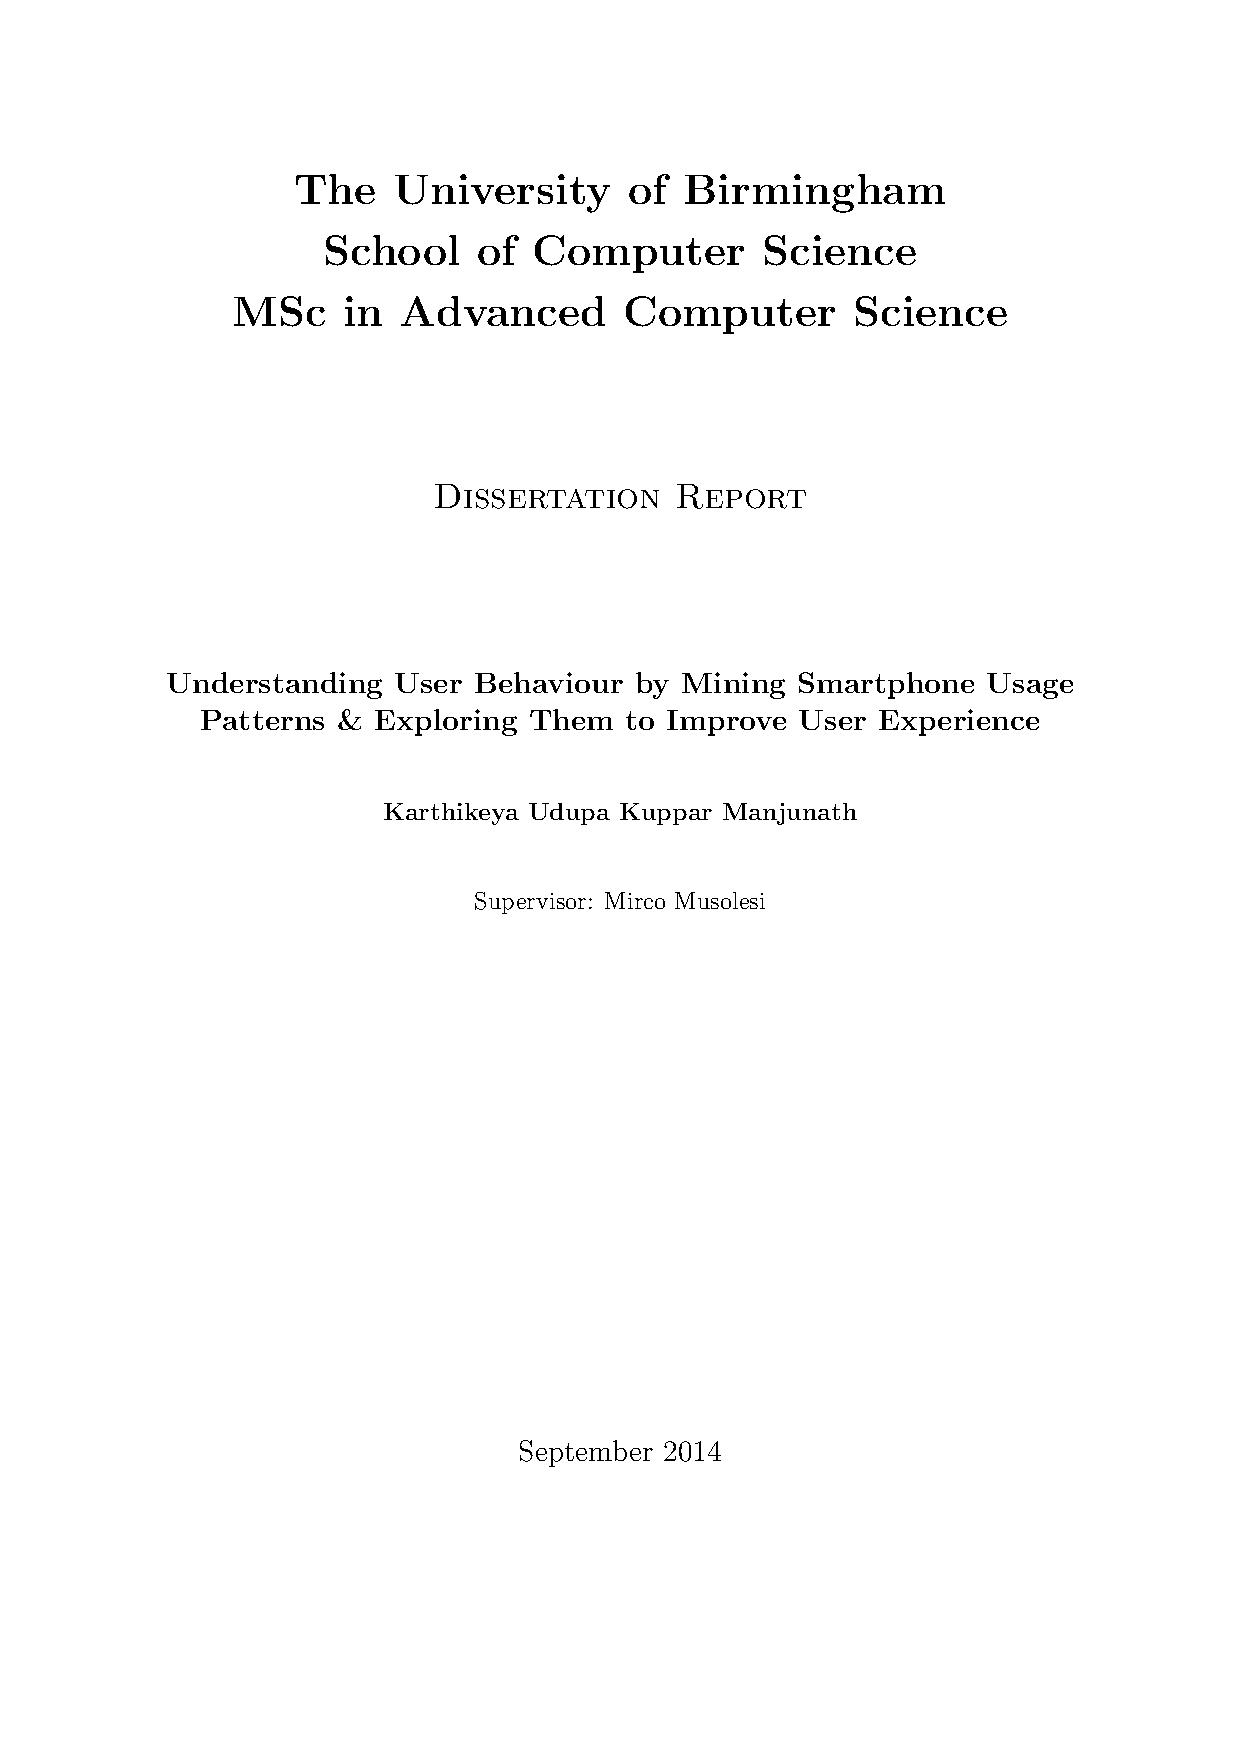
\includepdf[pages={1},scale=1.0]{cover_page.pdf}
% Title portion
\title{Understanding User Behaviour by Mining Smartphone Usage Patterns \& Exploring Them to Improve User Experience}
\author{Karthikeya Udupa Kuppar Manjunath
\affil{University of Birmingham}
Mirco Musolesi
\affil{(Supervisor) University of Birmingham}
Veljko Pejovic
\affil{(Supervisor) University of Birmingham}}

\begin{abstract}

\noindent
Mobility as a technology has seen advancement in the past two decades like no other rising to a level where it has become a necessity of modern day's daily life. From communication, entertainment to healthcare and fitness, mobile devices caters to all our needs in one way or other. Being such a key aspect of our lives, mobile presents us with interesting challenges that, if solved, can help improve our daily lives. 

The foremost goal of this research is to capture user's interaction with his smartphone and the applications on it and gather information about the contextual conditions that lead the user to perform the interaction in the first place. We then use the data gathered to look for interaction patterns and factors that can ultimately be used to improve user's experience with the mobile device. 

The research also aims at modelling the collected data which based on various factors, time and location among others, will try to predict application usage/application category usage. With the understanding of user behaviour, this model can further help us improve user’s experience. We also look at the modern day networking arena and provide a novel idea which would use \textit{Software Defined Networking} alongside the intelligence gathered from the data about application usage to provide a better networking solutions for the mobile users. We will also look into what further improvements can be made in the domain based on the evidence we have gathered which would further benefit the user.


\end{abstract}

%\category{C.2.2}{Computer-Communication Networks}{Network Protocols}

\terms{Mobile Architecture, Smartphone Monitoring, Smartphone Usage Analysis, Network Optimisation}

\keywords{Anticipatory System, Context Sensing Framework, Android, Smartphone Usage, Activity Monitoring, Network Optimisation, SDN, OpenFlow}

\maketitle


\section{Introduction}
Over the past decade, we have seen several technological advancements that have created a huge impact on the mobile platforms, allowing them to evolve not only to be more usable and reliable but also have made them economically feasible for the general masses making it a necessity in our day-to-day lives from being just a luxurious commodity. Trends in several emerging markets in the recent years have indicated that there is not only a tremendous increase in web activity originating from mobile platforms but also provides us a clear indication that the people are moving from traditional computing platforms to mobile devices, making mobile platform a very exciting and vital research area.

Smartphones and other wearable computing devices such as smart watches and glasses are the most recent additions in the field of mobile communication devices \cite{oulasvirta2012habits}. Even after being this recent, the overall smartphone penetration however has surpassed every possible expectation, from 46\% in 2012 it has now reached to 70\% penetration among adults in the US, all this within 7 years of the launch of popular smartphone such as iPhone \cite{smith201246,Asymco2012}. This rapid adaptation of smartphones throughout the masses is a clear indicator of not only its popularity but also the need it fulfills by empowering the users with communication capabilities, internet access, multimedia capabilities, navigation etc, justifying it as the most important technological advancement in the last decade \cite{ross2011top}.

These smartphones and other wearable technologies that have emerged recently have blended into out lives to become an extension of ourselves, allowing us to look into the the revolutionary ideas proposed by pioneers in this field in a new light \cite{weiser1991computer}. They also get a glimpse of who we are, the minute decisions that we take everyday, our preferences in terms of shopping, dinning, travel or even in the people that we meet, ultimately helping us to manage and simplify our daily lives and focus on important things then getting entangled in managing technology. 

However, various technologies that we use in parallel with the mobile platform still are being developed and setup as they were before. This although provides a working model of, but hinders the boost mobility can really provide. One such area is the networking platforms \cite{lee2014mesdn}, mobile networks still work on a traditional networking systems with not many significant upgrades for mobile or smartphone specific network. Similarly other areas such as web content delivery also can be improved. We will look into this further in this research.

From a research point of view, this level of adaption of ubiquitous technologies which can give us such good insight provides us the means to achieve more in terms of understanding user's behaviour in his natural environment. Not only is this wide network of devices a source of limitless contextual information \cite{campbell2008rise} but also provides us with a way to help improve daily life of the user by considerably reducing the efforts one puts in operating the technology yet allowing him to enjoy the benefits of the technology in his day-to-day life. 

However using smartphone as a research platform has its own demerits \cite{keshav2007cell,falaki2011systemsens} from being able to provide only restricted access for development and device data to just the sheer diversity available in the smartphone market; making it hard for a single application to capture the data for the masses. This research we would try to overcome the barrier of developing a monitoring application for the Android platform with certain level of reusability for future research. It would be looking into application usage patterns for Android using an application developed called \textit{WebSense} and try to find usage patterns which can help us further build a model to predict application usage among various other things. We would also be looking into a few possible uses to improve user's experience on the mobile phone using the prediction especially in the networking domain with the help of modern networking technologies such as \textit{Software Defined Networking}.

\section{Data Collection: Context Framework, \textit{WebSense} and Data Processing}
\label{collection}

Mobile platforms have various barriers when it comes to using them for research purposes. Each mobile platform comes with its own development framework, which makes it impossible to develop a piece of software which would flawlessly work on multiple platforms without any change. The platforms themselves have their own set of restriction on what contextual information can be monitored and what data that is being generated by the phone or the apps that are installed can be accessed. There are additional hassles such as ensuring compatibility of the application over the various devices that are available which work on that platform For example, iOS from Apple does not allow applications to monitor user application usage and web usage, both of which are very critical for this research. Android platform is considerably open and allows one to access various different kinds of contextual markers and app usage patterns. It also holds a majority among the masses in terms of mobile marketshare \cite{gartnerMobileSurvey2013}, making it a more suitable candidate to use for our research.

An essential part of this project is to develop and improve the process of gathering contextual information from real world users along with a way to monitor interactions on the mobile device on a day-to-day basis in an un-moderated environment. There are three essential aspects that need to be focused on to achieve this goal. Firstly, a framework which is used to gather contextual information from any Android based device. This framework was developed as a library for anyone to use in future research with minimal code to start monitoring contexts for their purposes. We will be discussing this further in section \ref{csf}.

The second component is the \textit{WebSense} mobile application, which is the front-end application that was mass-deployed on the \textit{Android Play Store} allowing people to participate in the research. The app's primary goal was to allow collection of information while proving a front-end which would provide user useful information to provide value to the user. The third component is the web server responsible for storage and maintaing of the data along with providing methods to extract useful information for further research. 

Although these components were developed to an extent in our previous research(see Appendix \ref{APX:previousWork}) but various large scale changes were made in the way of their functioning and several performance improvements were made that allowed fixing of crashes and provided stability to the application; issues that were detected using ACRA crash logging system that was added into the application were also fixed during the research. In addition to this the web component which was just collecting data previously was developed further to do various other tasks that we would be discussing in section \ref{ws}. 

\subsection{The Context Sensing Framework}
\label{csf}

\textit{Context} is an essential part of any system that tries to understand user behaviour or monitor user interaction. Monitoring usage context is a vital component in our research as well as it provides us with the insight and the understanding of the user's condition when he performed an certain activity.

Context itself has been defined and revised by many researchers over the course of time partly because of the definition's need to take into consideration the advancements in technology and what can actually be achieved in the reality which was not possible when it was not known earlier. The most recent and probably the most apt definition of context is that ``any information that can be used to characterise the situation of an entity. An entity is a person, place, or object that is considered relevant to the interaction between a user and an application, including the user and applications themselves.'' \cite{dey2001understanding}. This definition clearly outlines what we are trying to achieve with the framework.

The Framework was developed for Android platform after taking into consideration its openness in terms of data it is able to provide the overlaying application. Although there are several monitoring frameworks for Android \cite{lathia2013smartphones,novakextensible2013} however they all lack several vital components that are essential to our research such as application monitoring, web usage monitoring, network connections, WiFi access points among others.

Based on the platform restrictions, the sensors and the available APIs a set of contextual markers were selected to be collected, each type of context had its own process of extraction and reporting back.

\begin{itemize}
\item \textbf{Application Usage} - Application usage is the primary context that we are monitoring for this research. The framework provides information such as what app the user is using, for how long and meta-data about the app such as application name, package name, icon information etc. The process used to extract this information is by constantly scanning the device at fixed interval(4 seconds) and to look for changes. This information is propagated back to the app which is using the framework in the form of an \textit{Intent Broadcast}.

\item \textbf{Web Usage} - Web usage is derived from app usage, whenever the user is using an application which falls into the browser category and updates the data in the android browser database, the web browsing instance is observed. This is in the form of an URL and the duration it has been since the user moved to the page.

\item \textbf{Location Monitoring} - Location context is monitored in a very effective manner (see Appendix \ref{APX:previousWork}), proving a robust and fairly reliable process in providing location data to be used by the app. The polling duration and the provider can be customised based on the needs.

\item \textbf{Power Consumption} - Power consumption is monitored in terms of battery power that is left, since polling the battery is not an effective way to do it, the framework constantly listens for battery update notification from the OS and then uses that data to calculate details and then sends over in the form of a broadcast. Several fixes were made to handle faulty power readings in the previous version.

\item \textbf{WiFi Connectivity \& Nearby Access Points} - WiFi connectivity of the device allows us to check if the device is ready to be connected to WiFi, if it is connected to an access point and if there are other access points nearby. The details of other access points along with their signal strength is also recorded. In the previous versions the scans were too frequent creating large scale record sets for WiFi and also repeaters for the same access-points were considered, this along with several minor issues were fixed.

\item \textbf{Network Signals \& Nearby Towers} - Network signals provide the connectivity status of the device with the GSM/CDM network. The strength of the connection along with nearby access-point details is also captured and provided back to the integrated application.

\item \textbf{Bluetooth Status \& Nearby Devices} - Bluetooth connectivity status of the device tells us if the device has bluetooth switched on or not. It also lets us know if the device is paired and what are the nearby devices, all of which can be used to predict co-location among other social networking patterns between users. The device is scanned and also a system broadcast provides updates to the framework at regular intervals.

\item \textbf{Telephony Status} - The telephony status lets us know if the user is in a calling status or not.

\item \textbf{User's Events (Real world activities)} - Real world activities that are recorded by the user on his calendar such as meetings are monitored. This allows us to look into the user behaviour based on his real world condition. The information is scanned at a certain interval, any updates are sent to the connected app in the form of notification.

\item \textbf{Screen Status} - The status of the screen, if it is switched on or off is monitored and reported back. Off screen generally denotes inactivity of the user.

\item \textbf{Data Connectivity Status} - connectivity status of the device to the internet using 3G, 2G, Edge or GPRS is monitored.

\item \textbf{Mobile Device Settings} - Details about the devices various settings such as volume settings, brightness settings, manufacturing details, timezone is all monitored under the settings context.

\end{itemize}

The platform relies on a model of \textit{Broadcast-Receiver}, any application using the framework would have to subscribe to the context framework's instance for receiving update about the particular context it wants to monitor along with the frequency of the updates it requires.

The framework's architecture and the broadcast receiver models are further explained in the appendix \ref{APX:previousWork}.

\subsection{\textit{WebSense} - Front End Application}

Although framework provides a robust groundwork to collect information, a font-end application is essential for the collection of the data for research purposes. The application that was developed for this purpose was \textit{WebSense}. It was essential for the app to provide some valuable information as well so users would have an incentive to download it.

The application does two essential things, firstly it collects contextual information using the Contextual framework described in section \ref{csf}. However this information on local device is not that useful so it has to be synced to the server where further processing of the data can be done, we will discuss this further in section \ref{ws}.

The second important role of the application was to provide user some value in return of providing the data. Since this application was to be distributed on the App Store having a value was very essential. This requirement was completed by adding Application Trends screen which showed applications that were popular in the geographical vicinity and Web trends showing websites popular in the geographical vicinity. In addition to this it also allowed the user to monitor his app usage trends allowing him to identify the time spend on a particular app during the day/week/month.

The app was developed to a rudimentary level in the previous research, however it required several changes and improvements to actually function to its full potential and be deployed in the app store. Further the app was modified to accommodate the changes that were done to the sever and to the framework. You can read further about the internal functioning of the app and the development methodology in Appendix \ref{APX:previousWork}.

\subsection{Web Server Component}
\label{ws}

The web server component is responsible for storing all the information that the user's device provides in the required format. In the initial research a basic server was developed to provide API for storage and to accumulate data and provide statistics based listing for app usage trends.

The server constitutes of a \textit{Node.js} backend component combined with \textit{MongoDB} to store the information. The component store the required information coming from the app and various derived data into the various \textit{collections}, which are NoSQL's version of tables.

\begin{itemize}

\item \textbf{User Information} - Information about the registered users along with their device information. This also includes information required to login and maintain multiple session on various devices. This also stores information about the user's \textit{Office} and \textit{Home} tags that we would discuss further in section \ref{geotagging}.

\item \textbf{Application Usage Information} - The application usage instances generated while being used by various users is stored after some processing, that includes cleansing of the data, updating the application listing record from Google Play Store. The information constitutes of application's package name, active time, launch time (time of the day), location information, Geohash tags and generated tags for location among others.

\item \textbf{Web Usage Information} - The collection of all the instances of web usage by the user. This includes any record of web usage generated by the android system recognised browser (which writes data into android browser's database). The URLs are also scanned for meta data prior storing it into the collection.

\item \textbf{Contextual Information} - Contextual information about the user gathered by the application is stored in a single place, i.e., all the various context markers are stored together but are tagged accordingly along with location tags for easy extraction.

\item \textbf{Application Metadata} - Meta data collected from scarping application information on the store, primarily used for analysis of the kind of application to allow sorting of apps into categories. Other useful facts such as publisher, downloads, ratings etc are also captured. A web component and an API to perform this task was developed and can take any valid package name and fetch information accordingly.

\item \textbf{Web Metadata} - Metadata about scrapped websites based on the user's browsing activities, includes information such as title, some content and images, this is used for generating the trends screen on the device.

\end{itemize}

\subsection{Deployment, Collection \& Processing of App Usage Data}

The application after development and several cycles of revisions and fixes was deployed to the \textit{Android Play Store} with the backend deployed on a secure University of Birmingham server. The deployed application was downloaded by people around the world and data was accumulated over the period of time. The detailed analysis of the data is discussed further in section \ref{anadata}.

The collected data that is stored after being processed at various different levels; For example the application usage records are cleansed by removing unwanted keys that are being passed, then each record is checked against existing application records in the meta data collection and in case it is not present the meta data is downloaded through the meta data API that was created for this purpose. 

Location information which is available as coordinates makes it hard to work with so it was converted into a format which would work well with the custom processing algorithms. Additionally information such as \textit{Geohash} is generated as well, use of which we will be discussing further in this section. Similar process is applied to the context information as well.

\begin{figure}[hbtp]
 \centering
 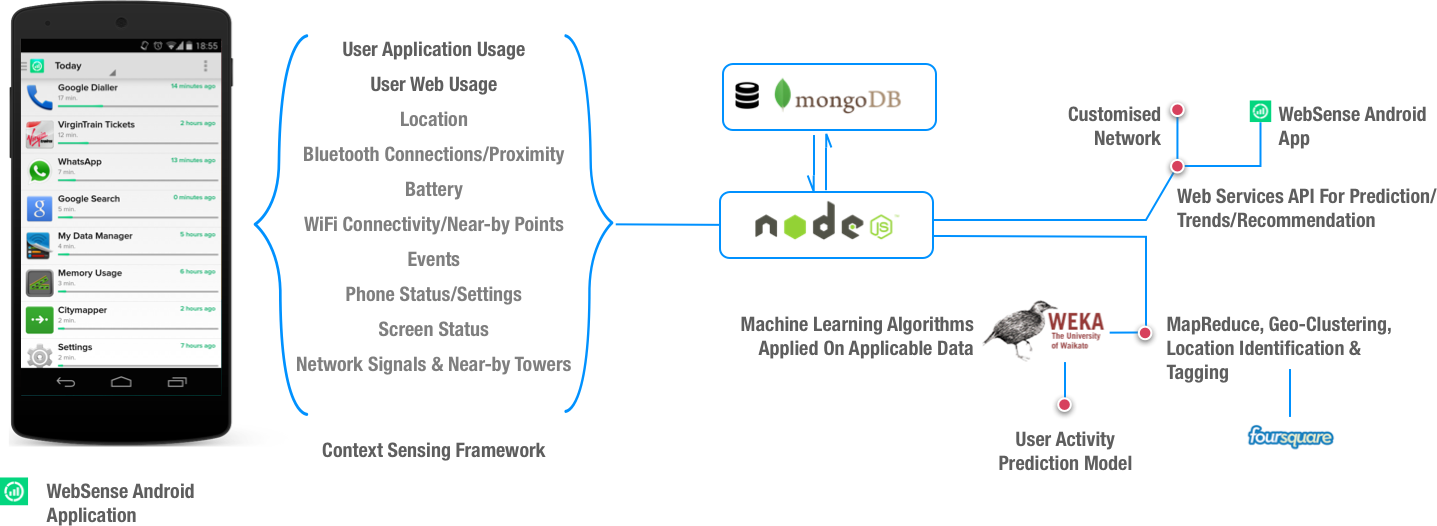
\includegraphics[width=120mm]{app_flow.png}
  \caption {Overall data processing and flow of information.}
 \label{fig:dataflow}
\end{figure}

In previous work (refer to Appendix \ref{APX:previousWork} for detailed information) we have used the basic data processing techniques to generate pattern with the help of standard \textit{MapReduce} algorithm by reducing usage duration over application package-name and then geofencing the data over a particular radius (location information of the user). Although this method did provide some useful information on possible trends and served well for providing useful information back to \textit{WebSense} app as a value add, but further analysis was done by utilising various other aspects of the data such as calculating trends information based on the time of the day the application was being used (local-time) and this was also combined with the location. This process was converted into API methods to be used in future systems that we would be discussing further in section \ref{networkdesign}.

Further we also looked into categories the application being used belonged to and associated it with the various times of the day and tried to extract useful information. The category of application being used is fetched from the app info collection that was generated whenever new applications are registered by the system, this allows to identify more meaningful patterns then just with a single applications.

Location being one of the most important contextual information was also analysed further to establish a relation if location has any significance on the apps being used by the user. However location itself might be irrelevant when we are considering multiple user's data once as geographical locations might be separated but still might have the same significance. For example a person who goes to office in London and a person who goes to office in Birmingham are both going to Office which in turn would have similar contextual implications. So inferring logical location instead of coordinate based location is important to analyse the result in the case of crowd-sensed data.

\subsubsection{Geo-Clustering of Data \& Location Tagging}
\label{geotagging}

The application usage data is tagged with geographical information (provided that the information was provided by the user's device and the location services were turned on by the user) however the location is in the form of latitude and longitude which in itself is a problematic type of information to process using traditional clustering algorithms. A technique was developed to process the data for easy use with MongoDB's inbuilt algorithms to provide clustered data that could be analysed further.

\textit{Geohash} is a geocoding system for converting coordinate into a compact string format; it designed by Gustavo Niemeyer. This provides us a very effective way to handle coordinate data in the database in a format which is also unique and can be used for further analysis in place of using latitude and longitude directly. The has is generated by interleaving bits of the latitude and the longitude, the obtained bits are converted into a string \cite{balkic2012geohash}. Each hash is a spatial bounding box which represents a certain geographical area; the longer the string is, more precise the location meaning the number of iterations of interleaving increases the accuracy, similarly if we remove the character (from the rear) the accuracy is reduced accordingly. 

\begin{figure}[hbtp]
 \centering
 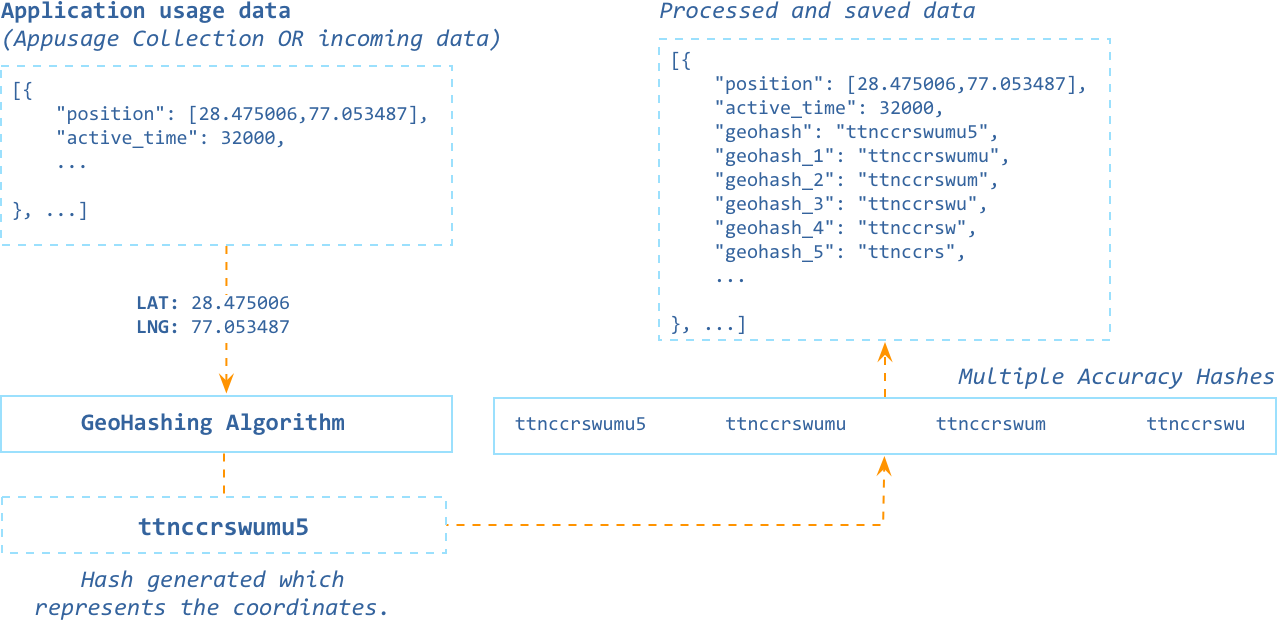
\includegraphics[width=120mm]{geohash.png}
  \caption {Process of marking Geohash with multiple accuracy levels.}
 \label{fig:geohashtablemap}
\end{figure}

Since the location is in a string format and we can scale the accuracy (see figure  \ref{fig:geohashtablemap}) by increasing or decreasing the length of the string it provides us with an very effective way to aggregate the location data. It is also to be considered that this method is not just reducing the length of the characters of longitude and latitude as that would be providing a very low precision in terms of result as we keep reducing accuracy to identify bigger clusters. Each incoming app usage record is processed and Geohash for multiple accuracy levels are generated and stored within the record itself, this only happens if the location data is available. All the data processing algorithms that need to use location then use this to reduce the dataset further. 

This proves very helpful when we need to process the data to identify critical location in user's life, for example home and work location of an user. As discussed identifying importance of location and tagging then would allow us to process the data for a group of user which can never be done with spatial coordinates. To identify the home and office location we analyse the app usage data, each app usage record consists of position/Geohash (coordinates and Geohash of multiple level), active\_time (duration of the app for that instance), package\_name(unique application identifier) and start\_time\_day (minute of the day at which the app got launched).

We cluster the application data by reducing the usage records over a period of time by accuracy level (hash with length 6, meaning a precision of .61km) using MapReduce algorithm, however this has be done based on time segments, so we consider two essential time segments, 0000 Hours to 0900 Hours and 0900 Hours to 1800 Hours of the day, these timings refer to the local time of the user and is not effected by the timezone he is in. These time windows would be the most probable time for people to be at home and work respectively (for most of the people, however exceptions might be there). 

Based on the information we have, we mapReduce application usage on a Geohash of a particular accuracy for an individual to identify two prominent points in his daily life. Home location should be relatively clear however office location might be somewhat inconsistent provided there are holidays and weekends so further cleaning of the data based on our knowledge of home location can help us identify a viable candidate for office location. Once these locations are identified we tag the applicable app usage records as \textit{Office} or \textit{Home} based on geohash, this allows us to tag records which are created at home or office during the wrong time period, i.e. weekend records during afternoon will be most likely be tagged as Home even though the time period is wrong, similarly people working late at office would be tagged Office even though the time window assumes that they are at home.

An API was built on top of this that allowed us to download the data in a format suitable for further processing using machine learning algorithms, this data would help us identify app usage patterns in office and homes and also will let us write prediction models which we will discuss further in section \ref{anadata}.

\begin{figure}[hbtp]
 \centering
 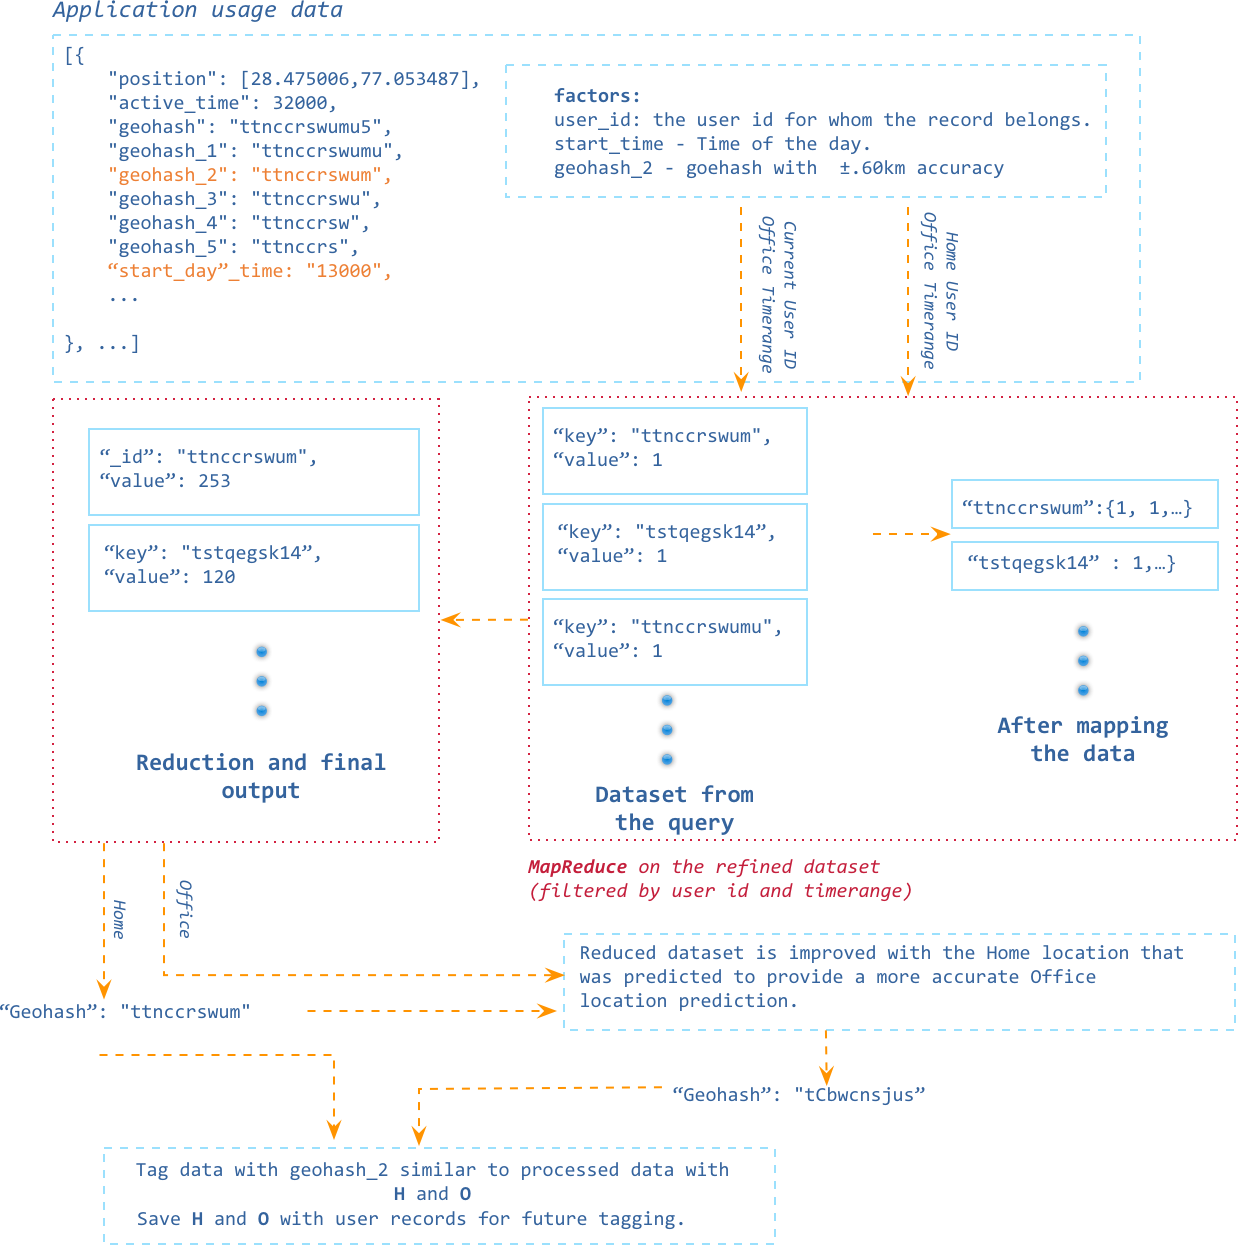
\includegraphics[width=120mm]{geo_home_office.png}
  \caption {Process of identifying home and office locations for a user and 
  tagging the app usage records.}
 \label{fig:HomeOffice}
\end{figure}


An interactive interface was created to analyse the extracted points further and not only to understand what the algorithm was really doing but also to analyse the results further visually (see figure \ref{fig:geohashclustering}).

\begin{figure}[hbtp]
 \centering
 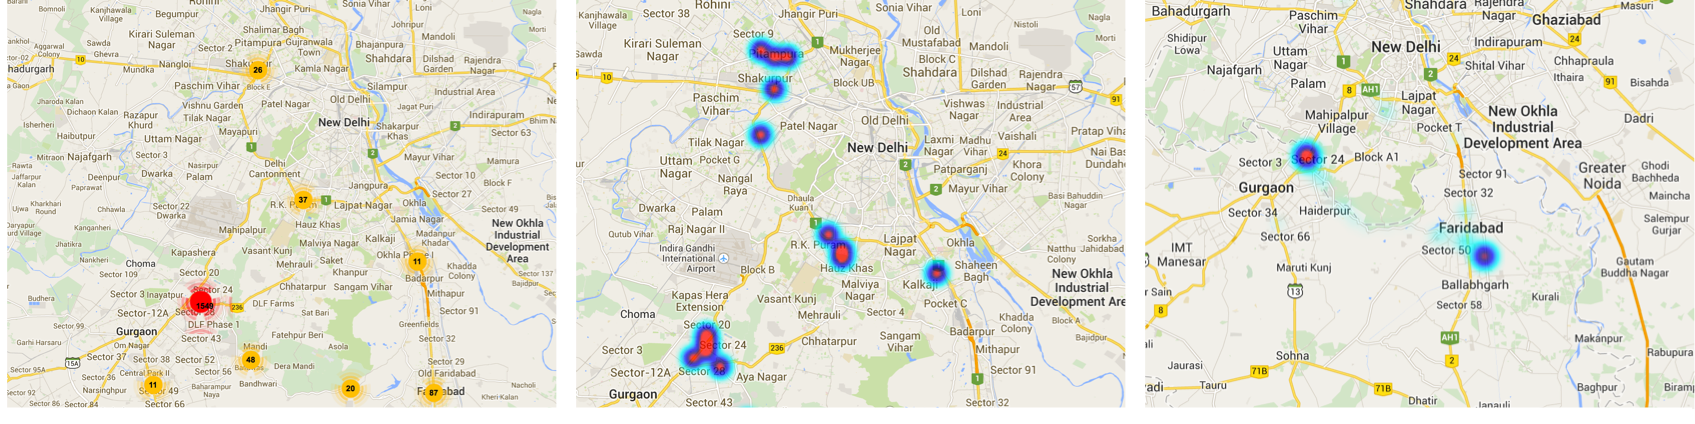
\includegraphics[width=120mm]{map.png}
  \caption {Heat-map and clustering visualisation based on Geohash based clustering, (i) Initial basic clustering based on coordinates. (ii) Heat-map of the clustered data. (iii) Heat-map after the algorithm for home and office detected has been executed.}
 \label{fig:geohashclustering}
\end{figure}

However, the tagging of office and home constitutes of a very small segment of the available app usage records, there are lot of other places that the users travel and possibly use apps at those locations, there can be some statistical significance or even a correlation between the application being used, the time and the nature of the location. However, we have the same problem as before, i.e., spatial location may vary but the context that the location provides might be similar for example a restaurant in London may provide the same kind of contextual condition as a restaurant in Birmingham. Hence we need to identify the nature of the location to derive a relation between location and the application being used. 

\begin{figure}[hbtp]
 \centering
 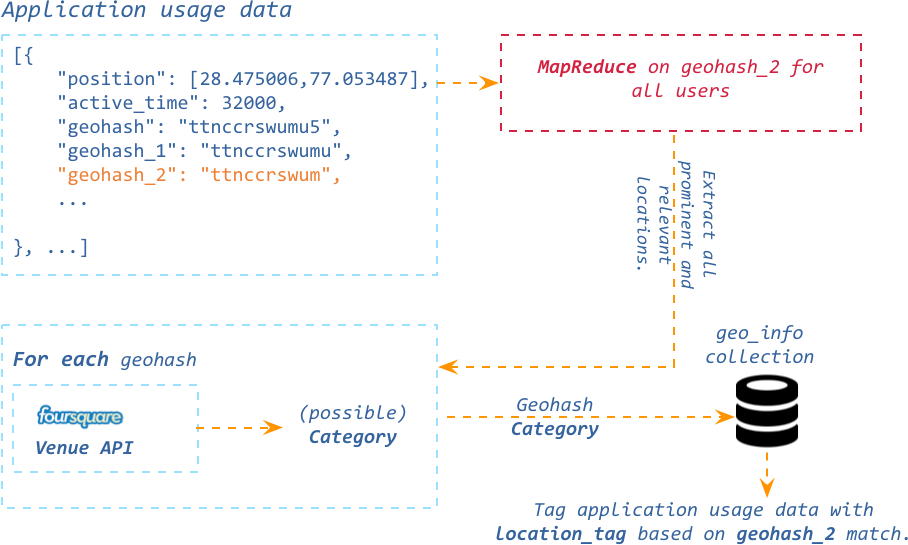
\includegraphics[width=120mm]{fsq_tagging.png}
  \caption {Tagging application usage records with location information.}
 \label{fig:appfsqtagging}
\end{figure}

To process this further we MapReduce application usage over a Geohash key of high accuracy to extract a set of prominent recurring points (to filter out only statistically significant locations) for all the users (we are also taking into consideration common places that people visited). This gives us a list of locations which can be further explored. \textit{Foursquare} provides various APIs\footnote{https://developer.foursquare.com/docs/ - Foursquare Developer API} which allows us to geocode location data and extract categorical information about locations; For example, we can identify a collection of points at Waterloo Station in London as \textit{``Tube Station''}. We process the set of locations that we discovered using the API to create a database of location and location category tags. This information is then used to tag application usage records with location tags. 

An API was built over it to download the data in a format for machine learning algorithms with application information, active time, launch time and location category. The overall process and the flow of the information is depicted in figure \ref{fig:dataflow}.

Considering this is a small scale experiment with a limited set of users the diversity of the location among the group might not be optimal, but this process still provides a novel approach to tag specified location clustering of data which can be further improved with a larger dataset with more accurate location information.


\section{Analysis of App Usage Patterns}
\label{anadata}

The \textit{WebSense} app once deployed on the \textit{Android Play Store} was downloaded and used by users worldwide who were also contributing in the form of data for app usage and contextual data. In this section we analyse the collected data and try to understand and draw meaningful observations from it. We also use the data to generate prediction models from the data.

The app overall had 22 users in total over a duration of 7 weeks, however it is to be noted that users have joined and left (uninstalled) the research, meaning it is not necessary that all the users would have a consistent 7 week of records. The overall records collected overall ~250,000 app interaction instances among the users and over ~2500 hours of user interactions being recorded. The application diversity is also very interesting, over the course of time the framework has gathered information/meta data of 270 applications, allowing them to be used to mark app usage instances along with categories. During this duration ~1950 URLs were browsed using the android recognised browsers.

\begin{table}[htdp]

\begin{tabularx}{\textwidth}{ XX }
 
  \textbf{Context Type} & \textbf{Record Count} \\
   \hline
   \\
  SIGNAL\_UPDATE\_NOTIFY  & 31586  \\
  WIFI\_UPDATE\_NOTIFY   & 452844  \\
  BLUETOOTH\_UPDATE\_NOTIFY   &  47712    \\ 
  BATTERY\_UPDATE\_NOTIFY  & 39511  \\
  EVENT\_UPDATE\_NOTIFY   &  144088    \\ 
  \\
   \hline
  \end{tabularx}
\\
\caption{}{\begin{center}Contextual record subdivision among the collected in contextinfo collection.\end{center}}
\label{contextcount}
\end{table}%


The contextual information that was gathered over the period is much more; with over ~700,000 among the users. The breakup of the contextual information is listed below in figure \ref{contextcount}.

From all the data that was gathered, we identified certain key components that were to be observed and with the help of various processes discussed in section \ref{collection} we filter the data.The following are some of the key components that were taken out for machine learning algorithms to process further.

\begin{itemize}
\item \textit{package\_name} - The name of the application package that is being used, this is a unique identifier for the app, several of the names have been been removed from set due to their association with the android system which makes them not a choice of the user. An example of this would be the android launcher.

\item \textit{category} - The category the application is assigned to by the developer. This information is scarped as a part of the meta-data collection when data is pushed to the server.

\item \textit{location\_tag (personal places)} - The location tag is the tag which specifies if the location is either \textit{Home} or \textit{Office}.

\item \textit{location\_tag (Public places)} - The location tag is the tag which specifies the outdoor location's significance based on the information fetched from the Foursquare API.

\item \textit{active\_time} - The local start time of the application interaction commencement. Represented as minutes.

\item \textit{day\_time} - the localised time of the day the user made that interacted in seconds, for example if the user interacts at 01:06 AM it would be recorded as 3601. This provides us an advantage, we can now compare data of users with the same time constraints wherever they are in the world.
\end{itemize}

\subsection{User's Application Usage Models}

Let us look into the Home and Office tagged users, out of the 22 users, 14 users had statistically significant data (others either did not have enough data or they did not provide location information making them irrelevant for this part of the study). Once the data is tagged we downloaded the data and ran it through a series of classifiers.

The goal of the models generated from this was the to predict the application usage based on time and location of the user, by location we mean the the local location\_tags. We ran a series of classifiers for 3 different sets of individual's data. The classifiers used were \textit{ZeroR}\footnote{ZeroR - http://weka.sourceforge.net/doc.dev/weka/classifiers/rules/ZeroR.html} as baseline, \textit{NaiveBayes}\footnote{NaiveBayes Classifier - http://weka.sourceforge.net/doc.dev/weka/classifiers/bayes/NaiveBayes.html}, \textit{Bayes Net}\footnote{BayesNet - http://weka.sourceforge.net/doc.dev/weka/classifiers/bayes/BayesNet.html} and \textit{J48}\footnote{J48 - http://weka.sourceforge.net/doc.dev/weka/classifiers/trees/J48.html}.

First set was the individual's set of \textit{Office} records, for the set of records we ran classifiers based on \textit{day\_time} to predict \textit{category}, the prediction highly depended on the data that was available for each of the user and also on the user's behaviour, from the various models being generated J48 usually had a very consistent prediction and was providing considerably better results then the baseline and other two classifiers (see Appendix \ref{APX:individual} for model's detailed summary). On an average J48 correctly classified an 80.26\% of the records in contrast to the 62\% by the baseline classifier, ZeroR. 

The second set of individual's \textit{Home} tagged records, however not all the users had a detected home due to lack of significant records, around 11 people were statistically significant for this modelling session. The classifiers were trying to predict \textit{category} based on \textit{day\_time}. The results (see Appendix \ref{APX:individual-Home}) as the previous one shows that J48 shows the most promising result of 71.11\% accuracy, however the difference from the baseline is not as much as before.

The third set is a combined set of \textit{Home} and \textit{Office} records of the individual, here the modelling parameters change, we try to now predict \textit{category} based on \textit{day\_time} and \textit{location\_tag}. Based on this we ran the classifiers, J48 provided  a consistently good performance with an average of 70.35\% with the baseline as 53\%.

The deviation in prediction however is high enough for us to understand that predicating user's activity even after several stages of classification still is very complex, additionally, based on the experience with erratic behaviour of the classifiers with instances with low number of record we can also conclude that the prediction can be improved provided that we have a larger dataset.

We also analysed the data as a group, meaning we combined all personally tagged data of the users and tried to derive an efficient model from it. For this we have 2 variations we can try, first set would be the to analyse the relation between the category and the time of the day app is being used, we will call it \textit{SET A} and the second set would be \textit{SET B} which will be for a relation between category with location tags and time.

\begin{table}[htdp]
\begin{tabularx}{\textwidth}{|X|X|X|X|X|}
\hline
\textbf{Data Set}      &\textbf{ZeroR}      & \textbf{NaiveBayes}      & \textbf{BayesNet}     & \textbf{J48}      \\ \hline
SET A & 64.07\% & 39.48\% & 82.59\% & 83.95\% \\
SET B & 35.93\% & 42.89\% & 82.54\% & 84.12\% \\
SET C & 38.80\%	& 38.38\% &	76.54\%	& 78.11\% \\ \hline
\end{tabularx}
\caption{}
\label{TBL:generalprediction}
\end{table}

With the collected data we ran multiple classifiers and built models, as you can see in Table
\ref{TBL:generalprediction}, on Set A we have a ~84\% predictability with the baseline at 64\% and on Set B the results are even better with a 85.12\% predictability with the baseline at ~36\%. Indicating a clear sense of predictability in this dataset, the dataset itself consists of around 60,000 records.

We also ran the series of classifiers on all the available data, regardless if they had location information or not to predict category based on time which we have marked as \textit{SET C} in the result. As we can see from the percentages of correctly predicted instances the predictability is substantial however when we compare it to SET B, i.e. with the location tag, predictability is considerably higher, implying that location plays a significant role in the application being used.

\subsection{Patterns in the Application Usage Data}

\begin{figure}[bhtp]
 \centering
 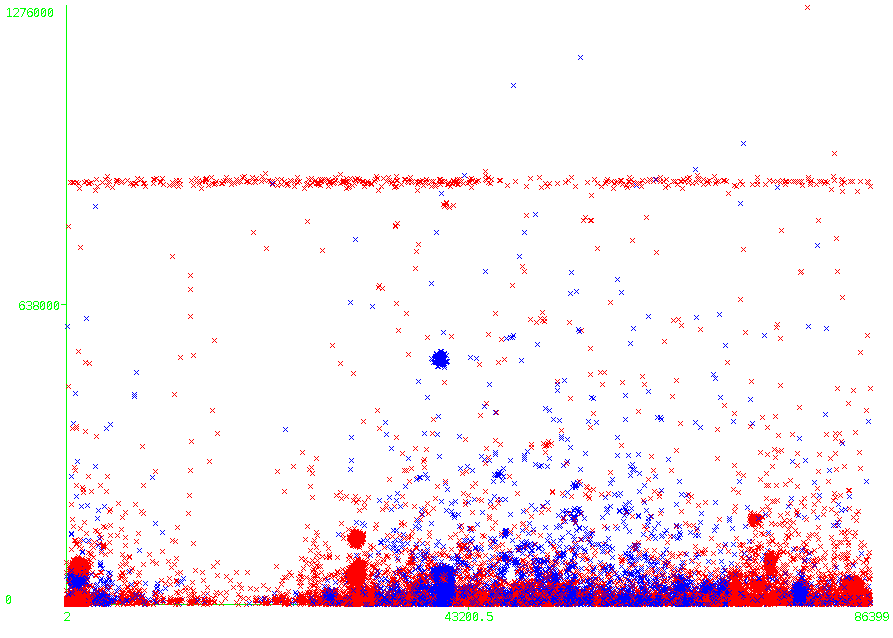
\includegraphics[width=80mm]{activity_start_time.png}
  \caption {Activity time throughout the day, red marks home instances and blue marks office instances.}
 \label{fig:appactivitytime}
\end{figure}

With the data we can identify several factors that influence various decisions in mobile design and can be used to help improve user interaction. Let us first look into active time of an application. It indicates how long an application is active before the user switches to another application or closes the app or the mobile locked itself. From the collected data we calculated the average for active time is around ~40 seconds, however there are cases of more then 2.5hour long interactions in case of multimedia and games applications. But the 40 seconds interaction windows actually provides us a glance into the overall attention span the user can spare per application at once, so applications should be developed to take into consideration that tasks should be complete-able within ~40 second window hence not making the task requiring more attention then the user can already spare. 

\begin{figure}[bhtp]
 \centering
 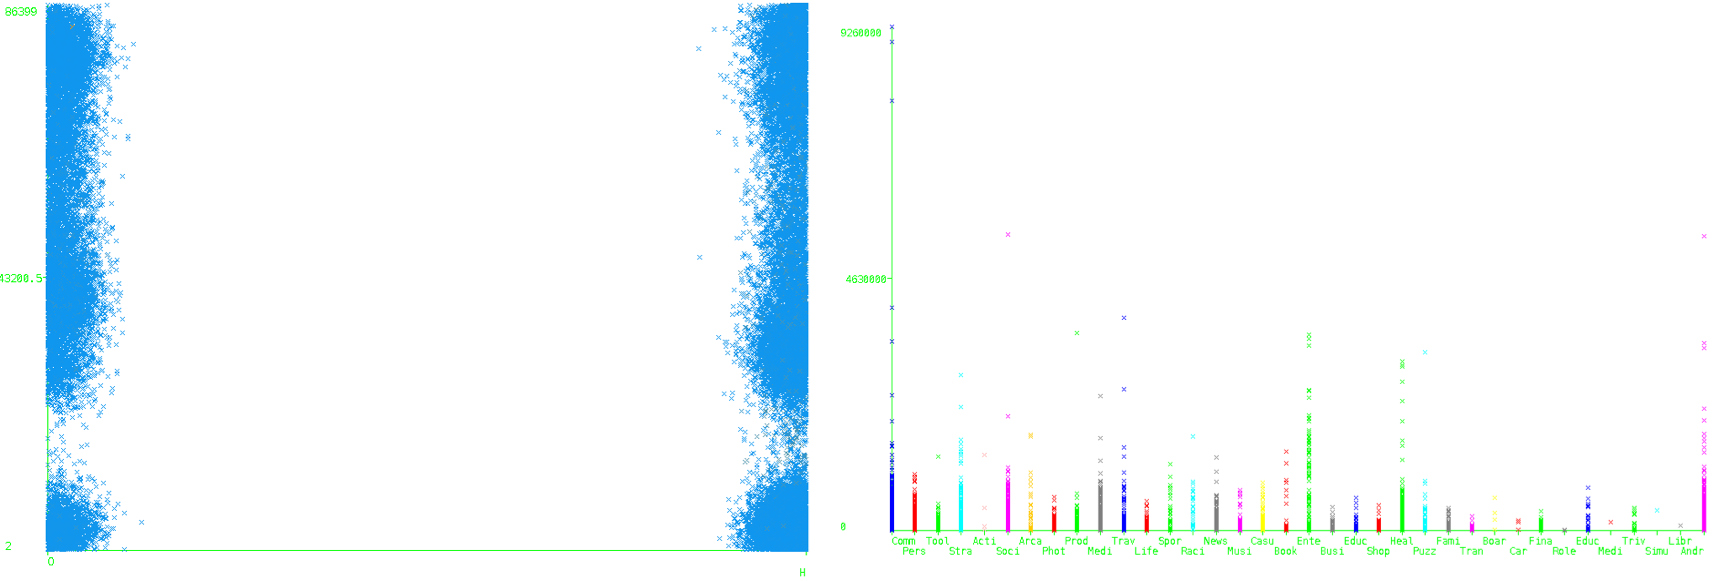
\includegraphics[width=120mm]{extra_graphs.png}
  \caption {Graphs showing different aspects of the data. (i) start time of the day with location tags, (ii) Various categories and active time of the app.}
 \label{fig:appextragraphs}
\end{figure}

When analysing active time we also found that there is a time duration of around 15 minutes where we can see a clear pattern in figure \ref{fig:appactivitytime} that throughout the day, applications tend to close here, The only possible cause of this can be concluded as screen turning off after 15 seconds. However, if that is the case, we can also see that there is a huge separation between user's app usage duration and the screen turn off time, we can hence reduce the screen switch off duration to around the same time as user's attention span in case of inactivity, the advantage being the battery being saved from turning off the screen. Using the available data we tried to sort app start time with location tag, we can see a pattern of people working late night at office and we can also see app usage pattern between office and home. We also can see the variation of active time between categories from which can understand that users spend more time on Entertainment, Communication, Social networking and Health and fitness application.

\subsection{Model for Generic Location Based Prediction}

From the available data we associated locations with categories as discussed in section \ref{geotagging} using Foursquare API. This gave us ~70,000 app usage records tagged with 104 distinct location categories and 27 distinct application types. To make the prediction more accurate we have already removed common repetitive system apps such as \textit{Launcher}, Android OS processes etc. We ran the the various classifiers that we used to predict category of application that one would use based on the location category and the time of the day. Furthermore we also tried to do the same prediction with just location type.

\begin{table}[htdp]
\begin{tabularx}{\textwidth}{|X|l|l|l|l|}
\hline
\textbf{Clustering Algorithm}      &\textbf{Set A}      & \textbf{Set B}      & \textbf{Set C}     & \textbf{Set D}      \\ \hline
ZeroR & 53.07\% & 53.07\% & 35.35\% & 24.26\% \\
NaiveBayes & 58.61\% & 63.12\% & 73.53\% & 47.67\% \\
BayesNet & 89.89\%	& 63.12\% &	73.58\%	& 88.00\% \\
J48 & 92.61\%	& 63.11\% &	73.62\%	& 90.11\% \\
J48Graft & \textbf{92.60}\%	& \textbf{63.11}\% & \textbf{73.62}\%	& \textbf{90.09}\% \\ \hline
\end{tabularx}
\caption{}
\label{TBL:fsqprediction}
\end{table}

Set 1 represents, category prediction with location tag and time, Set 2 is category prediction with location alone, Set 3 predicts package name based on location tag and set 4 predicts category based on location tag and time. As we can see the performance of J48 and J48 Graft is exceptional in most cases when compared with baseline. Set A and Set B which are the most significant predictions are also the most important ones. The ability to predict the category based on where the person is and what time it is can allow us to understand a co-relation between location and the apps. It also helps us prove that there is a similarity in the application usage pattern between different people at different locations but with the same significance (for example, different tube stations in different parts of the country).

With this kind of prediction we can take this further by caching information based on what we predict, this along with various other API's that are available we can change the way networks interact with the mobile devices. We will be discussing this further in the next section.


\section{Using the data to improve Network Design}
\label{networkdesign}

Networking has evolved over the years, from a simple Ethernet connection between machines to transfer information with the evolving needs of the industries and the consumers. Organisations require a networked environment using modern technologies such as Virtual machines acting as desktop and servers on cloud-based networks, data-storage devices in the cloud and automatically managing of permissions. But with increasing demands networks are getting complex by the day, there are requirements for improvement in quality of service, constantly changing traffic and requirement of complicated security policies that the network needs to comply with the traditional networks are getting harder to manage. 

These networking requirement are not only keep changing but also are very hard to comply with because of the way this has to be configured with networking devices such as routers and switches. Each manufacture would have their own way to configure it, making it hard for the administrators to follow thorough with the changes. And even if there is a way to do it on a device getting the change to propagate through the network on all the switches is nearly impossible because there is no standardisation among vendors and devices.

These problems make it nearly impossible for the networking to keep scaling at pace with the needs of organisations or network providers. Similarly is the case with mobile networks, from the analysis of the data in the previous sections we can clearly see the amount of interaction being performed by the mobile users on their respective devices is very significant. The amount of requests from the users is a constantly not only in the form of web pages but through the cloud based application that are available for these devices. This requires for a new form of networking that has to be more controllable and certainly more effective in providing content.

\subsection{Software Defined Networking}
The networking world has been experimenting with concepts which provide more control, flexibility in terms of dynamic rearrangement and configuration of the network, better moderation and easy management of policy groups with complex rules. One of the more explored way is with separation of control and data, this architecture of networks is known as Software Defined Networking or SDN. The concept relies on the ability to control the switches relatively easily. We separate the functionality of switches that support these architecture constitute of two layers or planes \cite{kirkpatrick2013software}, a data control plane responsible for forwarding incoming traffic to the required destination. The decision of forwarding the traffic however is taken by the control plane, it maintains flow table to forward traffic that it encounters.

The control plane provides control over traffic routing is also responsible for propagating policies. The data plane uses low end protocols such as UDP, TCP to transfer data. On a larger scale we can define SDN as a three tier architecture, at the bottom is the southern API, responsible for providing commands to help communication of behaviour of the network's switches, discovering the topology. OpenFlow\footnote{http://archive.openflow.org/} is the most common example of this. On top of this is the controller (POX, NOX, OpenFloodlight, OpenDaylight etc), providing its own API for the applications on top of it to allow application to control and reconfigure networks structure.
behalf of the applications \cite{paradis2014software}. Applications built on top of this are the ones who utilise the controllers methods to provide some useful functionality, prominent one being virtualisation ones \cite{alaettinoglu2013software}. 

\subsection{SDN and Mobile Devices}

SDN can create a huge impact on mobile devices by providing granular control over the network and its traffic. The challenge posed by the increasing requirements of the network can be solved by SDN networks with their dynamic management techniques to provide scalability and security in these networks which could not be traditionally achieved \cite{openflow2013}.

With the prediction and contextual data available and the research that have been done before we can look into several possible improvements.

\subsubsection{Predictive Caching with OpenCache \& OpenFlow}
The prediction API provides us the ability to predict application usage based on location and time. There are several API methods in the framework which can provide us with some kind of prediction for caching data.

\begin{itemize}
\item Application Prediction (Location, Time) - Prediction based on the location of access point and the time of the day. Can work with or without location or with or without time.
\item Application Prediction (Location Tags, Time) - Prediction based on the type of location the access point is on and the time of the day. Can work with or without location or with or without time. This uses the prediction model generated using J48 classifier in the section \ref{anadata}.
\item Web Prediction (Location, Time) - Prediction based on the trends of web usage based on location and time.
\end{itemize}

\begin{figure}[bhtp]
 \centering
 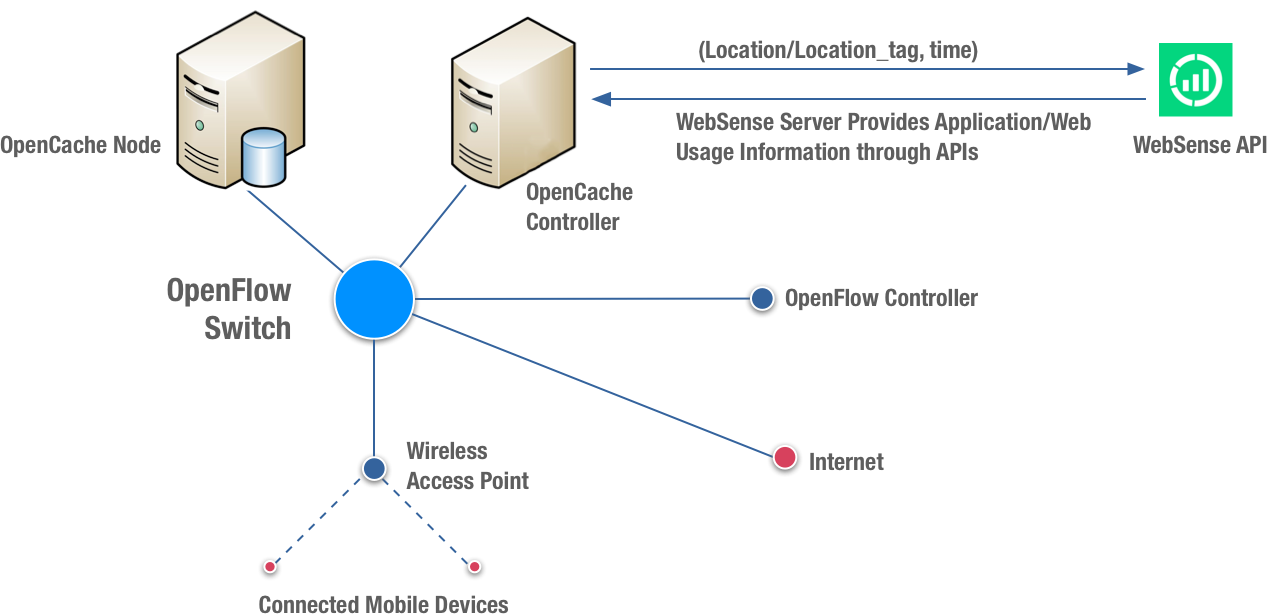
\includegraphics[width=120mm]{openflow-1.png}
  \caption {Predictive Caching Architecture.}
 \label{fig:openflowarch1}
\end{figure}

The application layer would implement a combination of OpenFlow and OpenCache \cite{broadbent2012opencache}. The OpenCache's node would be fed data from the prediction API and based on the prediction it would cache the content. The caching of content in an SDN network has already been proven effective \cite{chanda2013content} and the model itself has been proven in the section \ref{anadata} to provide satisfiable predictions, hence a combination of both would succeeded. The figure \ref{fig:openflowarch1} represents the mentioned architecture.

\begin{figure}[bhtp]
 \centering
 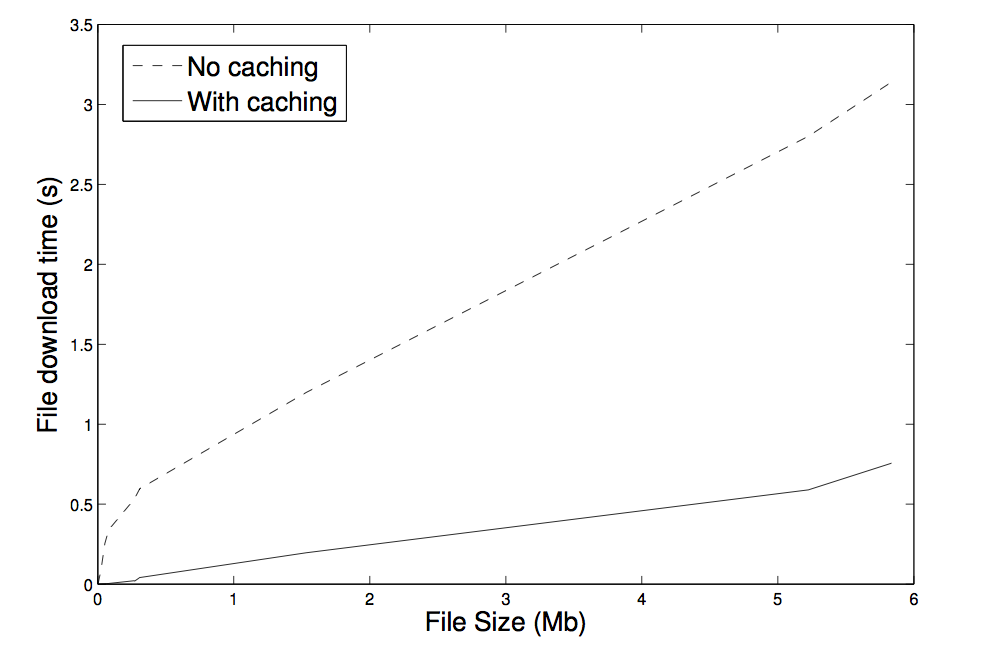
\includegraphics[width=80mm]{prediction_caching.png}
  \caption {Simple caching performance with SDN network \cite{chanda2013content}}
 \label{fig:openflowarch1predcaching}
\end{figure}


\subsubsection{Predictive Load Balancing and Improvement to Quality of Service}

The ability to monitor and control traffic in a network provides SDN with an opportunity to control how the network functions under increased load conditions or in case of network component failure. This allows us to improve the network's performance even in severe cases,  \cite{openflow2013} provides a keen insight into how Mobile traffic can be handled with the help of SDN and OpenFlow, it also points out off-loading technology, policy monitoring and failure handling.

The loading balancing feature activates if there is an increase or decrease in user network activity which would either strain the network or make free bandwidth available. The best examples would be public places, for example, a train station would have an increase in commuters during peak hours, which would mean that the networks in the vicinity would receive much more load and would require more bandwidth. Decisions can be taken to provide a consistent user experience, can either change its network configuration to handle more people or in certain cases alter its services, for example switch from 3G to 4G to increase its available bandwidth if the bandwidth in use exceeds a certain threshold hence maintaing the quality of service for the end user. Once the traffic reduces it can re-allocate resources accordingly.

The data that we have gathered provides a new perspective to this concept. With our data we can identify the dense user activity points, we can then look into the various time-windows during which the density increases or decreases and create a predictive model which suggests based time-window and location the level of network load the access-point would have and automatically scale the network beforehand providing a seamless transition before any actual load is put on the server. We also have the data for the cell-tower and wifi connections in the contextual info collection. This data can even be used to identify the connected towers and improve the network's performance accordingly. The figure \ref{fig:openflowarch2} represents the mentioned architecture.
\begin{figure}[bhtp]
 \centering
 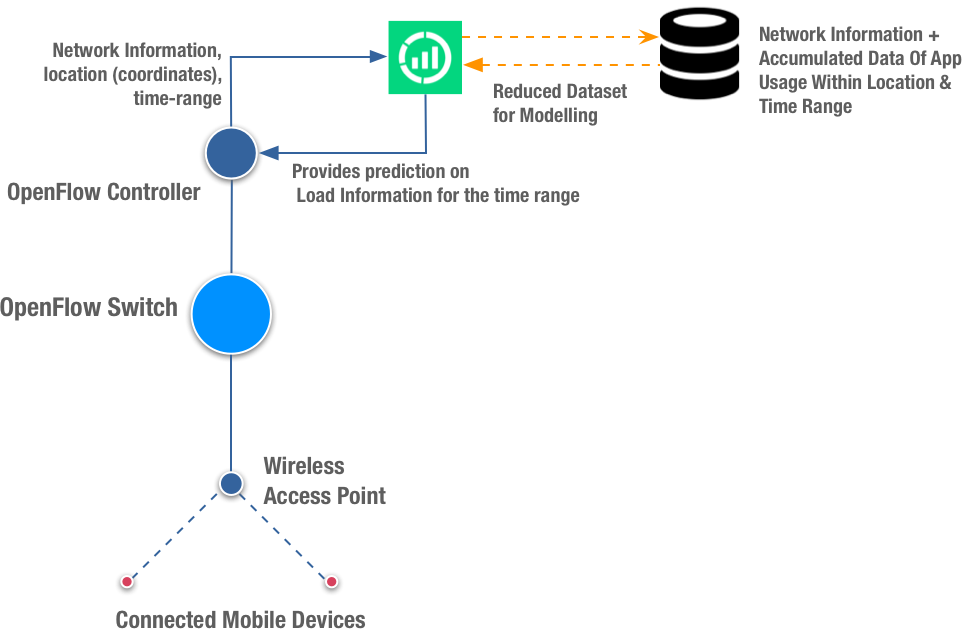
\includegraphics[width=120mm]{openflow-2.png}
  \caption {Predictive Load Balancing \& QoS Improvement Architecture.}
 \label{fig:openflowarch2}
\end{figure}

Additionally, we can use the data that we have about the application. For example, if the users tend to use VoIP applications more at a particular place, at a particular time, we can optimise the network's QoS and QoE (quality of experience) for the users \cite{2013aricent}. This would however require some change in the way the applications are designed; we would require additional meta data, either inside the application or from the Play Store about the nature of the application, kind of services it requires and even the URLs that can be cached. An example of this would be, Skype would come tagged with ``Service Type'' as ``VoIP'', games with networking requirement would come tagged as ``UDP'' and so forth so we would know before hand what the network has to be optimised to, we call this application-aware network \cite{2013aricent}. This can in theory be extended to http requests, for example, if a news app such as BBC is being used it might be tagged with the API url, we can cache the data accordingly. Other caching details such as for how long would that content be valid. 

If these changes are made available we can definitely improve the way networks are managed and change how they interact with mobile devices. Their ability to provide manage load and provide boosted performance to the apps/websites that are required or when there is an increase in traffic would improve the quality of experience people have on mobile

\section{Related Works}

The related work can be classified by various segments of the research. First segment that is the framework has had several efforts made on various platforms to develop a stable and reusable context sensing platform over the last few years. \textit{EmotionSense} project developed initially for Symbian 60 and now android focuses on monitoring context for the purpose of behaviour and emotions of the users \cite{rachuri2010emotionsense}. The framework provides various components such as adaptive sensing and broadcast based sensor information among other useful features. However, the android version being relatively new lacks several contextual markers that are readily available on the Android operating system.

Other platforms such as \textit{funf} provides dynamic sensing along with customisable saving options. Mobile Sensing Framework works with Ambient Dynamics allows customisation of contextual scanning dynamically \cite{novakextensible2013}. The framework also enables to mine and extract historical context that can be used in various ways.

The second segment is the monitoring of user application usage and other contextual markers to analyse and unearth important features in the data. A predictive launcher system called FALCON \cite{yan2012fast} provides predictive application launching services on Windows Mobile OS based on historical data of app usage that it gathers over the time along with other contextual markers. \cite{do2010their} mines a large scale collected data to understand various patterns and statistically significant relations between various factors much like what we are trying to do here. Another research  looks into the the various user activities and tries to derive implications based on the occurrence of various contextual factor and tries to build a user activity model with it.

\cite{oliver2010challenges} provides a similar research's finding on a totally different platform, \textit{Blackberry}. With a dataset of over 17000 users with over a millennium of user interaction time, it provides a very clear explanation to various factor in mobile research but it still lacks to understand the relation of individual application interaction which we have tried to achieve in this research. \textit{SystemSens} \cite{falaki2011systemsens} is also an interesting mobile architecture component built to analyse and research on mobile interaction, but it focuses on more system factors then user interaction such as power consumption and screen status, it does not give any focus to the user's specific interaction with the apps and webpages. Several other researches \cite{ferreira2011understanding,alawnah2013modeling} have focused on understanding the power consumption aspect, enabling us to understand and improve the situation of power consumption on mobile.
The networking aspect of the research has not been explored much probably due to the fact that SDN is still an emerging technology and is not widely deployed yet. However there are a few initial ideas that are trying to reinvent networking design using modern technologies like SDN and OpenFlow switches. \cite{chanda2013content} provides an architecture with practical implementation of an caching engine base on OpenFlow and SDN with proof for how caching can be improved with the help of SDN. Several white-papers have touched the subject of mobile based caching and load balancing in an Software defined network \cite{openflow2013,2013aricent}. This is just theoretical work and does a practical implementation. meSDN takes the research one step further with a practical implementation of SDN for mobile network with an application-aware network which helps improve the quality of service \cite{lee2014mesdn}, however, this does not consider the ability to predict in the caching or the predictive load balancing.


\section{Limitations \& Future Works}
There are several shortcomings in this research that we know of, however, each of them can be dealt with if provided enough time and resources. Firstly, the data collected is very limited, both in terms of the number of users and also in terms of the duration it was collected for. Additionally, the user group is relatively less diverse, i.e., it constitutes mostly of people in the range of 20-30 years and either work or study at universities, this creates a lot of discrepancies in the data such has no clear distinction in work and office location, less diverse applications being used, odd work hours etc. Additionally, the application had a few users who uninstalled application in between the study that led to several smaller user datasets which proved statistically insignificant in several cases.

The application was developed for gathering of the data with location as one of the aspects, however since location become a prime aspect of the study, a more accurate and frequently scanned location information would have been very helpful in deriving conclusions. This especially comes in handy when dealing with Foursquare APIs. Also, expanding the application's support to more devices and platforms would certainly help increase the dataset and the user-base. The foursquare tagging can be improved even further with better location data and by combining categories, at present it has diverse data which can be combined, for example, restaurants currently are tagged by types, i.e., indian, italian, persian etc. instead of being tagged as just restaurant.

The SDN model is another aspect that lacked certain features. Although it was well described in the sections above a fully working model with evaluation would certainly have proved vital to the research. Additionally having the meta-data about applications, which at present unfortunately is not available anywhere, would be helpful in providing increased quality of service to the users.

The SDN implementation of the caching engine with detailed analysis of the results and improvements it would be providing will certainly help us prove the usefulness of the architecture. A detailed model that uses application data along with network information would also help in providing the required data for the load-balancing architecture.

\section{Discussion}

Through this research we have tried to look into the various aspects of mobile computing; the activities that we participate in daily, which can be improved for the betterment of the overall mobile usage experience and reduce the strain technology puts on the user's daily life. 

The \textit{WebSense} application along with its architecture provides an innovative platform that can be used further to not only analyse application usage but to understand various other co-relations between various contextual markers. Similarly, the Context Sensing framework can act as the groundwork for future contextual research on mobile by driving the efforts of the researchers towards the real problem away from the technological barrier. However, this framework can certainly be improved and can adopt certain features from existing framework such as EmotionSense \cite{rachuri2010emotionsense} while retain its simplicity of usage.

We also looked into the gathered data and processed it with various in-built and custom algorithms to extract meaningful patterns in the data and also to model data based on location, location tags and time to predict application and category of the application that a person would use with a considerably high success rates using various machine learning algorithms. The duration or active\_time provided us with an insight into human attention span towards application and how it can be used in development of a less strenuous application. The predication results when used with the emerging networking technology, Software Defined Networking, in the proposed novel architectures certainly seems to be promising as shown by the  caching experiments and the prediction accuracy of the model, however a real world implementation would be required before we can further speculate its usability. QoS and load balancing technologies,     which are already in use alongside SDN can also certainly benefit from the dataset we have about application usage, migration patterns and network connectivity data.

We believe that mobile certainly holds the potential to change the people's lives and alter the way they interact with the world. With more and more increase in mobile usage we would certainly have to turn towards emerging technologies to meet our ever growing needs and to develop architectures which would not only make the user's experience on the mobile devices seamless but also introduce a simplicity in the way we interact with mobile, helping us focus on the real-life rather then be entangled with technologies.


% Bibliography
\bibliographystyle{ACM-Reference-Format-Journals}
\bibliography{Report_1_0}

% Electronic Appendix
\elecappendix

\medskip

\section{Individual Prediction Model}

\subsection{Office tagged model's correctly predicted instances \%}
\label{APX:individual}

\begin{table}[htdp]
\begin{tabular}{lllll}
\hline
\textbf{User}      &\textbf{ZeroR}      & \textbf{NaiveBayes}      & \textbf{BayesNet}     & \textbf{J48}      \\ \hline \\
User 1  & 41.67\% & 41.38\% & 56.60\% & 73.76\%  \\
User 2  & 57.81\% & 52.71\% & 99.99\% & 100.00\% \\
User 3  & 64.86\% & 70.27\% & 64.86\% & 70.27\%  \\
User 4  & 87.27\% & 83.64\% & 87.27\% & 90\%     \\
User 5  & 64.86\% & 70.27\% & 64.86\% & 86.49\%  \\
User 6  & 87.27\% & 83.64\% & 87.27\% & 90\%     \\
User 7  & 32.43\% & 58.11\% & 96.40\% & 100\%    \\
User 8  & 43.10\% & 45.61\% & 43.10\% & 53.14\%  \\
User 9  & 62.09\% & 63.51\% & 62.09\% & 69.67\%  \\
User 10 & 41.67\% & 42.11\% & 64.53\% & 86.23\%  \\
User 11 & 84\%    & 74\%    & 84\%    & 84\%     \\
User 12 & 43.48\% & 43.48\% & 43.48\% & 50.84\%  \\
User 13 & 85.42\% & 85.42\% & 85.42\% & 85.83\%  \\
User 14 & 83.89\% & 82.46\% & 83.41\% & 83.41\%  \\ \\ \hline 
\textit{Average} & \textit{62.84}\% & \textit{64.04}\% & \textit{73.09}\% & \textbf{80.26}\%  \\ \hline
\end{tabular}
\end{table}


\subsection{Home model's tagged model's correctly predicted instances \%}
\label{APX:individual-Home}
\begin{table}[htdp]
\begin{tabular}{lllll}
\hline
\textbf{User}      &\textbf{ZeroR}      & \textbf{NaiveBayes}      & \textbf{BayesNet}     & \textbf{J48}      \\ \hline
User 1  & 37.79\% & 37.79\% & 37.79\% & 42.77\% \\
User 2  & 49.70\% & 99.99\% & 43.02\% & 99.99\% \\
User 3  & 69.16\% & 68.92\% & 66.27\% & 72.53\% \\
User 5  & 73.33\% & 100\%   & 100\%   & 100\%   \\
User 6  & 38.75\% & 42.19\% & 38.54\% & 47.16\% \\
User 7  & 69.96\% & 70.08\% & 69.24\% & 75.51\% \\
User 8  & 52.69\% & 52.69\% & 52.41\% & 54.67\% \\
User 9  & 41.67\% & 56.60\% & 41.38\% & 73.76\% \\
User 10 & 70.93\% & 74.41\% & 68.37\% & 82.82\% \\
User 11 & 49.33\% & 50.67\% & 49.48\% & 49.63\% \\
User 13 & 84.92\% & 84.42\% & 81.41\% & 83.42\% \\ \hline 
\textit{Average} & \textit{58.02}\% & \textit{67.07}\% & \textit{58.90}\% & \textbf{71.11}\% \\ \hline 
\end{tabular}
\end{table}

\subsection{Office and Home tagged model's combined correctly predicted instances \%}
\label{APX:individual-Combined}
\begin{table}[htdp]
\begin{tabular}{lllll}
\hline
\textbf{User}      &\textbf{ZeroR}      & \textbf{NaiveBayes}      & \textbf{BayesNet}     & \textbf{J48}      \\ \hline
User 1  & 38.27\% & 38.27\% & 39.21\% & 43.15\% \\
User 2  & 39.65\% & 54.29\% & 99.99\% & 99.99\% \\
User 3  & 68.81\% & 69.03\% & 65.71\% & 72.57\% \\
User 5  & 32.43\% & 92.79\% & 58.11\% & 100\%   \\
User 6  & 39.38\% & 38.66\% & 41.72\% & 46.34\% \\
User 7  & 69.85\% & 69.15\% & 72.76\% & 76.83\% \\
User 8  & 54.85\% & 53.76\% & 54.74\% & 54.96\% \\
User 9  & 43.95\% & 43.99\% & 52.05\% & 66.09\% \\
User 10 & 72.03\% & 71.36\% & 74.54\% & 80.07\% \\
User 11 & 47.53\% & 48.15\% & 47.74\% & 49.59\% \\
User 13 & 85.19\% & 84.97\% & 85.19\% & 84.28\% \\ \hline 
\textit{Average} & \textit{53.81}\% & \textit{60.40}\% & \textit{62.89}\% & \textbf{70.35}\% \\\hline
\end{tabular}
\end{table}

\newpage
\section{Section 2}
\label{APX:previousWork}
The following sections are extracted from a previous work of ours submitted for the Mini research work at University of Birmingham. This explains the architecture of the software and the backend used in this project which was developed to an extend in the previous works.
\pagestyle{plain}
\includepdf[pages={15-34},scale=0.9,nup=1x2,landscape=true]{mini_project_report.pdf}
\end{document}